\documentclass[11pt,a4paper]{article}
\usepackage[utf8]{inputenc}
\usepackage[T1]{fontenc}
\usepackage[spanish,es-noquoting]{babel}
\usepackage[margin=2.5cm]{geometry}
\usepackage{amsmath}
\usepackage{graphicx}
\usepackage{booktabs}
\usepackage{float}
\usepackage{microtype}
\usepackage[hidelinks]{hyperref}

\graphicspath{{../figures/}{figures/}}
% generado por gen_numeros.py
\newcommand{\imgOneTopUno}{hog}
\newcommand{\imgOnePTopUno}{0.130}
\newcommand{\imgTwoTopUno}{beaver}
\newcommand{\imgTwoPTopUno}{0.259}
\newcommand{\imgThreeTopUno}{beaver}
\newcommand{\imgThreePTopUno}{0.498}
\newcommand{\stabMin}{0.872}
\newcommand{\stabMax}{0.979}
\newcommand{\cfgMaxEvals}{2000}


% A11 -- Dos entradas de nombres de los integrantes
\newcommand{\NombresUno}{Josué Emanuel Say García \quad Carné 22801}
\newcommand{\NombresDos}{Gustavo Adolfo Cruz Bardales \quad Carné 22779}

\title{\bfseries ¿El animal o el agua?\\[0.3em]
\large Explicaciones SHAP de un Vision Transformer preentrenado}
\author{\NombresUno \\[0.4em] \NombresDos}
\date{4 de septiembre de 2026}

\begin{document}
\maketitle

\begin{abstract}
\noindent
Explicamos con SHAP las predicciones de \texttt{deit-small-patch16-224}, un Vision
Transformer preentrenado en ImageNet-1k, sobre tres imágenes elegidas para separar dos
hipótesis: que el modelo se apoya en el animal, o que se apoya en el contexto acuático de la
escena. La misma especie recibe dos etiquetas distintas según el fondo: una capibara sobre
tierra seca se clasifica como \texttt{\imgOneTopUno} ($p=\imgOnePTopUno$), mientras que una
capibara en la orilla de un río se clasifica como \texttt{beaver} con $p=\imgThreePTopUno$,
casi el doble de confianza que la que el modelo asigna a una fotografía de un castor real
($p=\imgTwoPTopUno$). Los mapas SHAP muestran que en ese caso la atribución positiva hacia
\texttt{beaver} recae sobre la orilla y el agua, mientras que el cuerpo del animal contribuye
en contra. Concluimos que, para estas entradas, el contexto pesa más que la morfología.
\end{abstract}

\section{Caso y pregunta explicativa}

Un clasificador de imágenes puede acertar, o fallar, por razones que no tienen que ver con el
objeto que se le pide reconocer. Cuando el fondo está correlacionado con la clase, el modelo
puede aprender el fondo. Este trabajo examina ese riesgo con SHAP \cite{lundberg2017unified}
sobre un modelo preentrenado, sin entrenar nada.

\paragraph{Modelo.} \texttt{facebook/deit-small-patch16-224} \cite{hfdeit}, un DeiT-Small
\cite{touvron2021deit} de $\sim$22\,M de parámetros, preentrenado en ImageNet-1k
\cite{deng2009imagenet} y usado tal cual, con sus 1000 clases originales. DeiT es un Vision
Transformer \cite{dosovitskiy2021vit}, no una red convolucional.

\paragraph{Pregunta explicativa.} \emph{¿En qué regiones de la imagen se apoya DeiT para
asignar su etiqueta: en el cuerpo del animal o en el contexto acuático de la escena?}

\paragraph{Imágenes de prueba.} Tres, elegidas para que el contraste responda la pregunta
(figura~\ref{fig:entradas}). IMG-01 e IMG-03 son la misma especie —capibara— en contextos
opuestos, seco y acuático; IMG-02 es la otra especie en contexto acuático. Si el modelo mira
al animal, IMG-01 e IMG-03 deberían recibir etiquetas parecidas; si mira al contexto, IMG-03
debería parecerse a IMG-02.

\begin{table}[H]
  \centering
  \begin{tabular}{llll}
    \toprule
    ID & Contenido & Fuente & Licencia \\
    \midrule
    IMG-01 & capibara, tierra seca & \texttt{freds0/capybara\_dataset} & MIT \\
    IMG-02 & castor, nadando & iNaturalist, foto 725021665 & CC BY-NC \\
    IMG-03 & capibara, orilla de río & iNaturalist, foto 721783385 & CC BY-NC \\
    \bottomrule
  \end{tabular}
  \caption{Las tres entradas analizadas. Las URL exactas están en \texttt{results.json} y en
  la segunda celda del notebook.}
\end{table}

\begin{figure}[H]
  \centering
  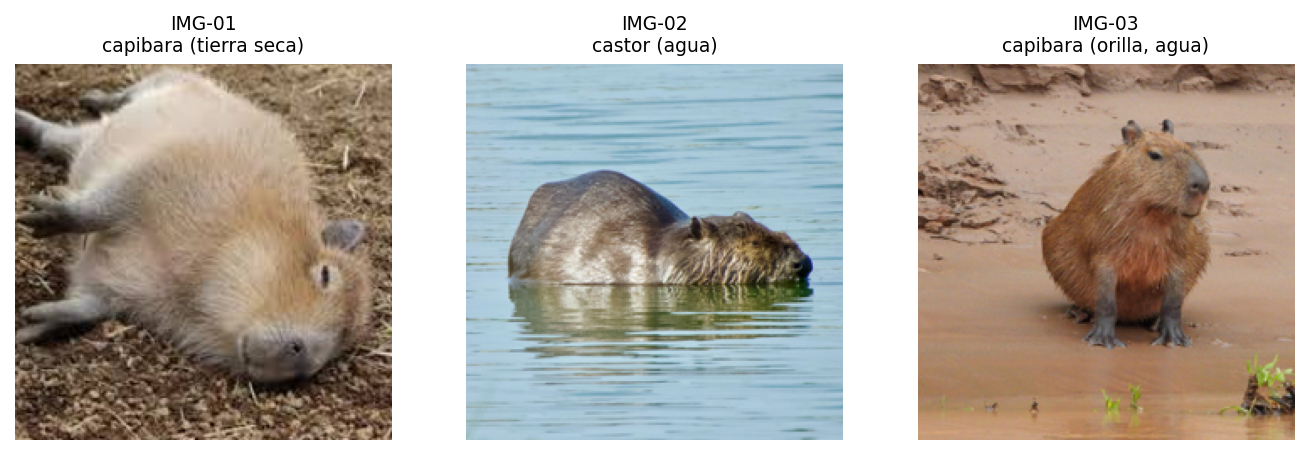
\includegraphics[width=\textwidth]{entradas.png}
  \caption{Las tres imágenes tal como las recibe el modelo, tras \texttt{Resize(256)} y
  \texttt{CenterCrop(224)}.}
  \label{fig:entradas}
\end{figure}

\paragraph{Nota sobre el vocabulario del modelo.} ImageNet-1k contiene la clase
\texttt{beaver} (índice 337) pero \textbf{no} contiene \texttt{capybara}. El modelo no tiene
cómo nombrar correctamente una capibara, así que para IMG-01 e IMG-03 devolverá
necesariamente una etiqueta equivocada. Lo que nos interesa no es el acierto, sino
\emph{en qué se apoya} para responder.

\section{Método}

Como DeiT no es convolucional, los explicadores de SHAP basados en gradientes por capas
(\texttt{DeepExplainer}, \texttt{GradientExplainer}) no aplican. Usamos el explicador
model-agnóstico \texttt{shap.Explainer} con \texttt{shap.maskers.Image} (algoritmo
\emph{Partition}), que trata el modelo como caja negra: perturba regiones de la imagen y mide
el cambio en la probabilidad de salida.

El \emph{baseline} de enmascarado es la imagen desenfocada (\texttt{blur(128,128)}) y no un
parche gris o negro, para no introducir estructura fuera de distribución que el transformer
interpretaría como contenido. La elección del baseline cambia los valores de Shapley: no es
un detalle cosmético. Presupuesto: \cfgMaxEvals\ evaluaciones por imagen.

\paragraph{Criterio de lectura, fijado antes de ver los mapas.} Hay evidencia de que el
modelo \emph{mira al animal} si la atribución positiva a la clase predicha se concentra sobre
el cuerpo o la cabeza; de que \emph{mira al contexto} si cae sobre regiones de agua,
vegetación u orilla sin animal. Un resultado mixto se reporta como mixto.

\section{Resultados}

\begin{table}[H]
  \centering
  \begin{tabular}{llcc}
    \toprule
    ID & Contenido real & Etiqueta predicha & $p$ \\
    \midrule
    IMG-01 & capibara, tierra seca  & \texttt{\imgOneTopUno}   & \imgOnePTopUno \\
    IMG-02 & castor, nadando        & \texttt{\imgTwoTopUno}   & \imgTwoPTopUno \\
    IMG-03 & capibara, orilla       & \texttt{\imgThreeTopUno} & \imgThreePTopUno \\
    \bottomrule
  \end{tabular}
  \caption{Predicciones del modelo preentrenado. Ninguna capibara puede clasificarse bien
  porque la clase no existe en ImageNet-1k; lo informativo es la diferencia entre IMG-01 e
  IMG-03, que contienen la misma especie.}
  \label{tab:preds}
\end{table}

El resultado central está en el cuadro~\ref{tab:preds}. \textbf{La misma especie recibe dos
respuestas distintas según el fondo}: sobre tierra seca, el modelo dice
\texttt{\imgOneTopUno}; en la orilla de un río, dice \texttt{beaver} con
$p=\imgThreePTopUno$. Esa confianza es además mayor que la que el modelo asigna a la
fotografía del castor real (IMG-02, $p=\imgTwoPTopUno$): la capibara en el agua le parece más
un castor que el propio castor.

\begin{figure}[H]
  \centering
  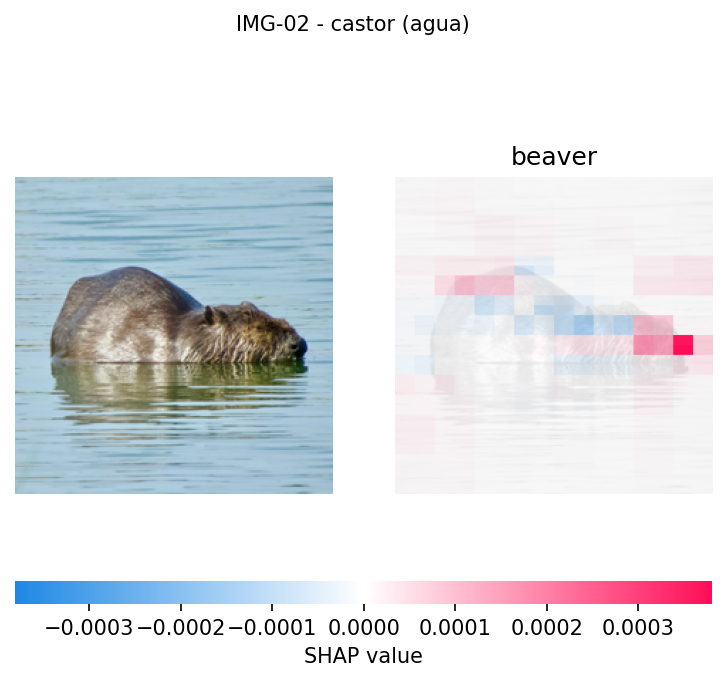
\includegraphics[width=0.49\textwidth]{shap_img-02.png}
  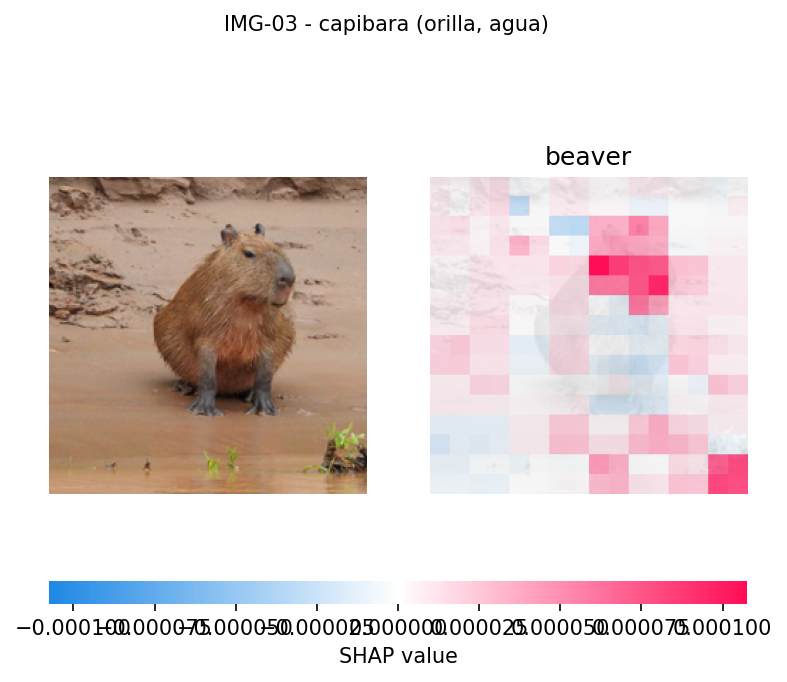
\includegraphics[width=0.49\textwidth]{shap_img-03.png}
  \caption{Atribuciones SHAP hacia la clase predicha. Izquierda, IMG-02 (castor real).
  Derecha, IMG-03 (capibara en la orilla): la atribución positiva hacia \texttt{beaver} se
  reparte por la orilla húmeda y el agua del borde inferior, mientras que buena parte del
  cuerpo del animal recibe atribución \emph{negativa}, es decir, contribuye en contra de la
  etiqueta que el modelo termina eligiendo.}
  \label{fig:shap}
\end{figure}

La figura~\ref{fig:shap} responde la pregunta explicativa para estas entradas. En IMG-03 el
modelo no llega a \texttt{beaver} por la forma del animal —el animal empuja en dirección
contraria— sino por el entorno. Conforme al criterio fijado de antemano, esto es evidencia de
que \textbf{mira al contexto}.

\begin{figure}[H]
  \centering
  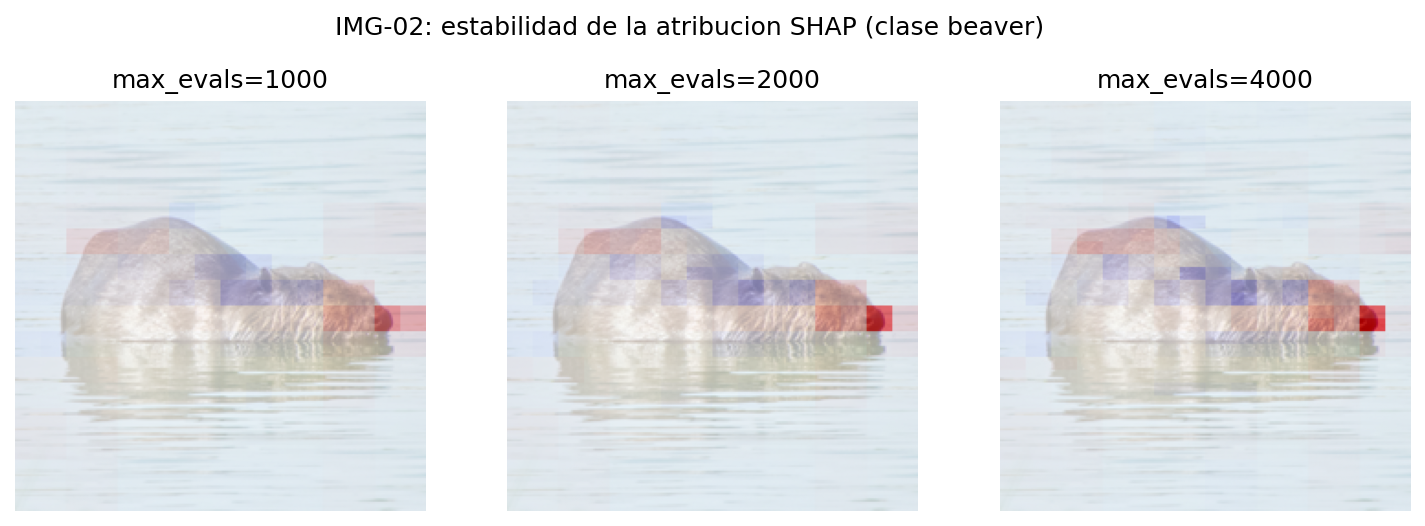
\includegraphics[width=\textwidth]{estabilidad.png}
  \caption{IMG-02 explicada con tres presupuestos de evaluación. La estructura gruesa se
  mantiene; el detalle fino cambia, por lo que no interpretamos bordes finos del mapa.}
  \label{fig:estabilidad}
\end{figure}

\paragraph{Estabilidad.} \emph{Partition} es una aproximación con presupuesto finito, así que
un mapa no comprobado no autoriza a afirmar que una región importa. Repetimos IMG-02 con 1000,
2000 y 4000 evaluaciones (figura~\ref{fig:estabilidad}): la correlación de Pearson entre los
mapas resultantes va de \stabMin\ a \stabMax.

\section{Limitaciones}

\begin{enumerate}
  \item \textbf{Tres imágenes no generalizan.} Son casos ilustrativos elegidos por diseño, no
  una muestra representativa. No medimos con qué frecuencia ocurre este comportamiento.
  \item \textbf{El modelo no puede acertar en dos de las tres entradas.} \texttt{capybara} no
  existe en ImageNet-1k, así que parte del error observado es una limitación del vocabulario
  y no necesariamente un atajo aprendido. Ambas explicaciones son compatibles con los datos
  que tenemos.
  \item \textbf{Sesgo geográfico y de hábitat.} Castores y capibaras viven en continentes
  distintos y en escenas visualmente distintas; el fondo está correlacionado con la especie
  por construcción del problema. Un mapa que resalte el agua es por tanto ambiguo entre
  «atajo» y «señal legítimamente correlacionada».
  \item \textbf{SHAP es aproximado y depende del baseline.} Los valores no son los de Shapley
  exactos y cambiarían con otro enmascarado o resolución \cite{kumar2020problems}. La única
  comprobación de validez que hicimos es la de estabilidad; no aplicamos los tests de
  aleatorización de Adebayo et al.\ \cite{adebayo2018sanity}.
  \item \textbf{Asociación, no causalidad.} Un mapa SHAP relaciona regiones con la salida del
  modelo; no establece un mecanismo causal.
  \item \textbf{Un error de implementación detectado y corregido.} En una primera ejecución,
  las dos fotografías de iNaturalist se guardaban con el mismo nombre de archivo local, de
  modo que IMG-03 reutilizaba la imagen de IMG-02 y ambas producían resultados idénticos. Se
  detectó al revisar que las probabilidades coincidían exactamente, se corrigió y se
  reejecutó todo. Las cifras de este documento provienen de la ejecución corregida.
\end{enumerate}

\section{Conclusiones}

Volviendo a la pregunta explicativa: para estas tres entradas, DeiT preentrenado se apoya de
forma sustancial en el contexto de la escena y no en la morfología del animal. La evidencia
es que la misma especie recibe dos etiquetas distintas según el fondo, que la capibara en el
agua se clasifica como \texttt{beaver} con más confianza que un castor real, y que en ese
caso el mapa SHAP sitúa la atribución positiva en la orilla y el agua mientras el cuerpo del
animal contribuye en contra.

Con tres imágenes no puede afirmarse que el modelo se comporte así en general, y la ausencia
de \texttt{capybara} en su vocabulario es una explicación alternativa que estos datos no
descartan. Lo que sí muestra el ejercicio es que una predicción puede parecer razonable
—\texttt{beaver} para un roedor semiacuático en el agua— y sostenerse sobre las regiones
equivocadas, algo que la etiqueta por sí sola no deja ver y que SHAP sí.

\section*{Reproducibilidad}

El notebook \texttt{shap\_deit.ipynb} ejecuta todo: descarga las tres imágenes por URL, carga
el modelo, calcula las atribuciones y guarda las figuras y \texttt{results.json}. Corre en
Google Colab o en local; en CPU tarda unos 8 minutos. Las cifras de este documento se generan
automáticamente desde \texttt{results.json} hacia \texttt{numeros.tex}, de modo que el texto
no puede desincronizarse de la ejecución.

\bibliographystyle{plain}
\bibliography{refs}
\end{document}
